\documentclass[11pt]{article}

\usepackage{course}
\begin{document}

\ctitle{1}{Decision trees and k-Nearest Neighbors}{Jan 30, 2018 at 11:59 pm}
\author{}
\date{}
\vspace{-1in}
\maketitle
\vspace{-0.75in}

\blfootnote{Parts of this assignment are adapted from course material by Andrea Danyluk (Williams), Tom Mitchell and Maria-Florina Balcan (CMU), Stuart Russell (UC Berkeley), Carlos Guestrin (UW) and Jessica Wu (Harvey Mudd).}

\ifsoln
\else
\section*{Submission instructions}
\begin{itemize}
\item 
Submit your solutions electronically on the course Gradescope site as PDF files.
\item If you plan to typeset your solutions, please use the LaTeX solution template. If you must submit scanned handwritten solutions, please use a black pen on blank white paper and a high-quality scanner app.
\end{itemize}
\fi

\ifnotsolution{\newpage}
\section{Splitting Heuristic for Decision Trees \problemworth{20}}
Recall that the ID3 algorithm iteratively grows a decision tree from the root downwards. On each iteration, the algorithm replaces one leaf node with an internal node that splits the data based on one decision attribute (or feature). In particular, the ID3 algorithm chooses the split that reduces the entropy the most, but there are other choices. For example, since our goal in the end is to have the lowest error, why not instead choose the split that reduces error the most? In this problem, we will explore one reason why reducing entropy is a better criterion.

Consider the following simple setting. Let us suppose each example is described by $n$ boolean features: $X = \langle X_1, \ldots, X_n \rangle$, where $X_i \in \{0, 1\}$, and where $n \geq 4$. Furthermore, the target function to be learned is $f : X \rightarrow Y$, where $Y = X_1 \vee X_2 \vee X_3$. That is, $Y = 1$ if $X_1 = 1$ or $X_2 = 1$ or $X_3 = 1$, and $Y = 0$ otherwise. Suppose that your training data contains all of the $2^n$ possible examples, each labeled by $f$. For example, when $n = 4$, the data set would be
\begin{table}[H]
\centering
\begin{tabular}{cccc|c}
$X_1$ & $X_2$ & $X_3$ & $X_4$ & $Y$\\ \hline
0 & 0 & 0 & 0 & 0\\
1 & 0 & 0 & 0 & 1\\
0 & 1 & 0 & 0 & 1\\
1 & 1 & 0 & 0 & 1\\
0 & 0 & 1 & 0 & 1\\
1 & 0 & 1 & 0 & 1\\
0 & 1 & 1 & 0 & 1\\
1 & 1 & 1 & 0 & 1\\
\end{tabular}
\quad \quad \quad \quad
\begin{tabular}{cccc|c}
$X_1$ & $X_2$ & $X_3$ & $X_4$ & $Y$\\ \hline
0 & 0 & 0 & 1 & 0\\
1 & 0 & 0 & 1 & 1\\
0 & 1 & 0 & 1 & 1\\
1 & 1 & 0 & 1 & 1\\
0 & 0 & 1 & 1 & 1\\
1 & 0 & 1 & 1 & 1\\
0 & 1 & 1 & 1 & 1\\
1 & 1 & 1 & 1 & 1\\
\end{tabular}
\end{table}

\begin{enumerate}
\item \itemworth{5} How many mistakes does the best $1$-leaf decision tree make over the $2^n$ training examples? (The $1$-leaf decision tree does not split the data even once. Make sure you answer for the general case when $n \geq 4$.)

\solution{}
The best $1$-leaf decision tree would just assign 

\item \itemworth{5} Is there a split that reduces the number of mistakes by at least one? (That is, is there a decision tree with $1$ internal node with fewer mistakes than your answer to part (a)?) Why or why not?

\item \itemworth{5} What is the entropy of the output label $Y$ for the $1$-leaf decision tree (no splits at all)?

\item \itemworth{5} Is there a split that reduces the entropy of the output $Y$ by a non-zero amount? If so, what is it, and what is the resulting conditional entropy of $Y$ given this split?

\end{enumerate}

\section{Entropy and Information \problemworth{5}}
The entropy of a Bernoulli (Boolean 0/1) random variable $X$ with $p(X = 1) = q$ is given by
\begin{equation*}
B(q) = - q \log q - (1 - q) \log(1 - q).
\end{equation*}
Suppose that a set $S$ of examples contains $p$ positive examples and $n$ negative examples. The entropy of $S$ is defined as $H(S) = B\left(\frac{p}{p+n}\right)$.
\begin{enumerate}
\item \itemworth{5} Based on an attribute $X_j$, we split our examples into $k$ disjoint subsets $S_k$, with $p_k$ positive and $n_k$ negative examples in each. If the ratio $\tfrac{p_k}{p_k + n_k}$ is the same for all $k$, show that the information gain of this attribute is 0.

\end{enumerate}

\section{k-Nearest Neighbors and Cross-validation \problemworth{15}}
In the following questions you will consider a $k$-nearest neighbor classifier using Euclidean
distance metric on a binary classification task. 
We assign the class of the test point to be the
class of the majority of the $k$ nearest neighbors. 
Note that a point can be its own neighbor.
\begin{figure}[h]
    \centering
    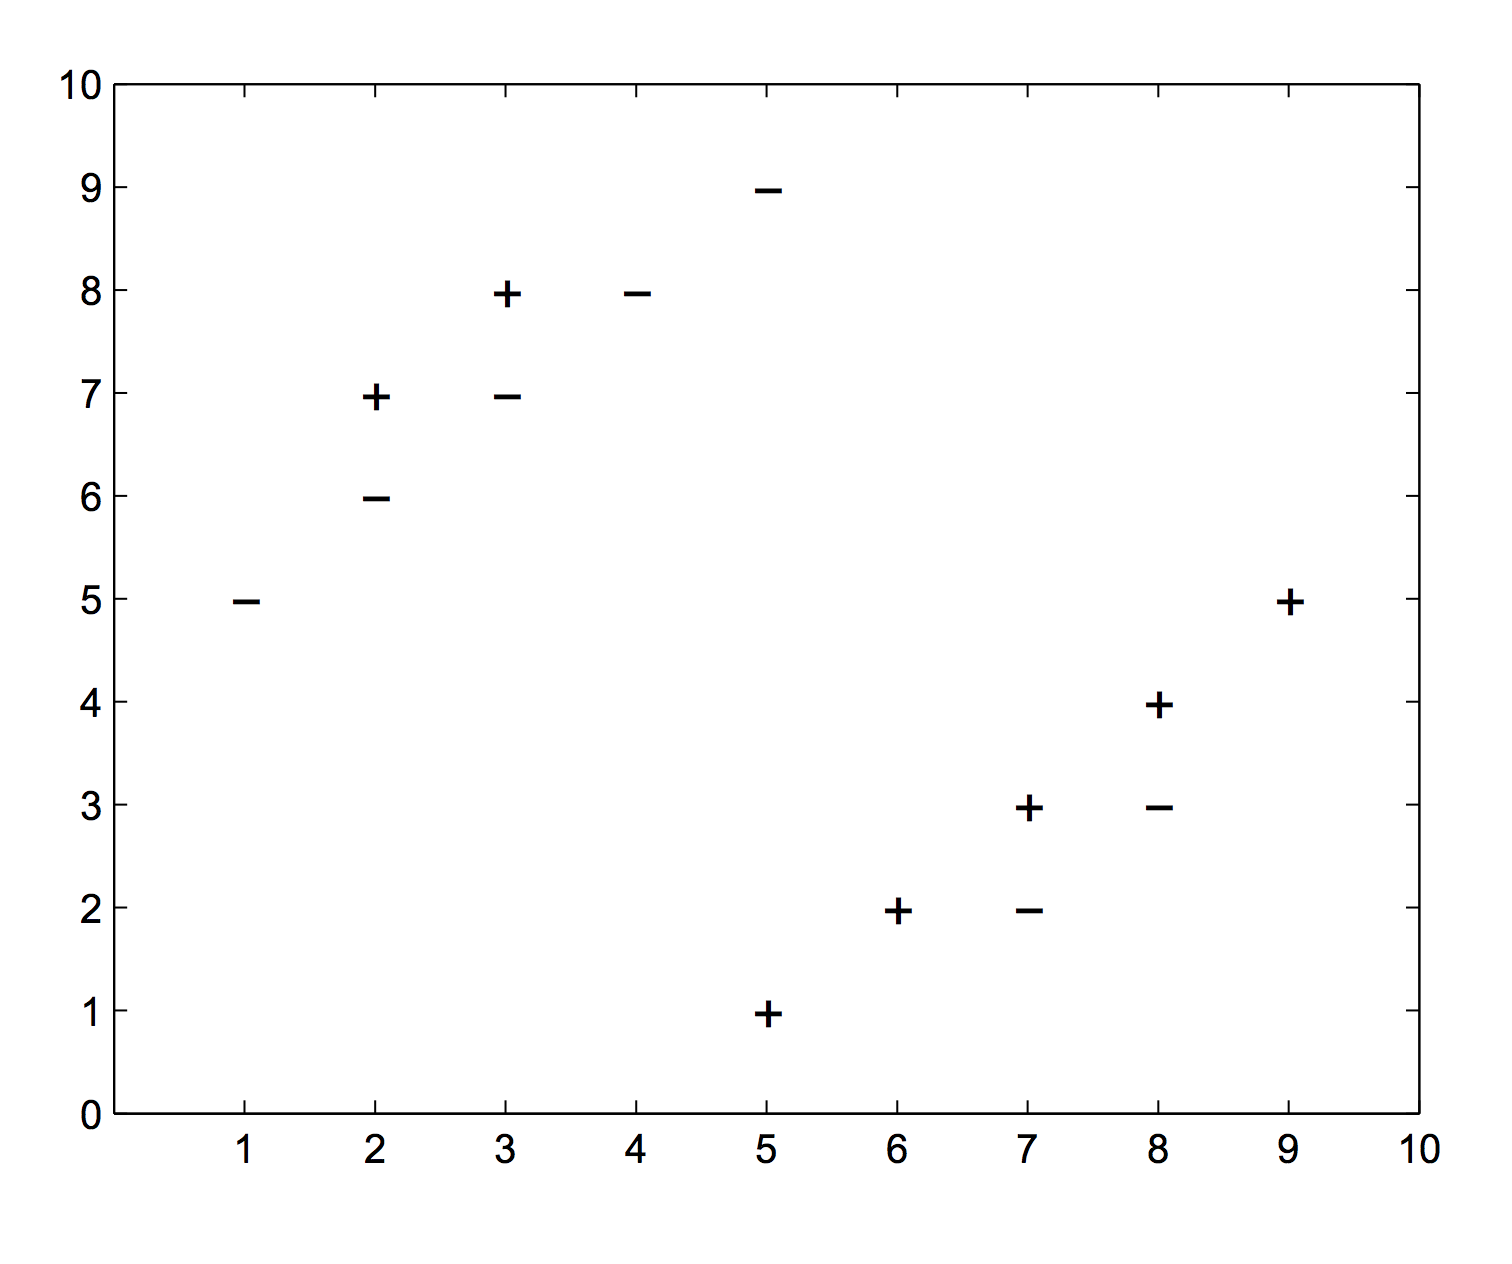
\includegraphics[scale=0.45]{knn_figure.png}
    \caption{Dataset for KNN binary classification task.}
    \label{fig:knn}
\end{figure}

\begin{enumerate}
    \item \itemworth{5} What value of $k$ minimizes the training set error for this dataset? What is
the resulting training error?
    \item \itemworth{5} Why might using too large values $k$ be bad in this dataset? Why might too
small values of k also be bad?
    \item \itemworth{5} What value of $k$ minimizes leave-one-out cross-validation error for this
dataset? What is the resulting error?
\end{enumerate}
\section{Programming exercise : Applying decision trees and k-nearest neighbors \problemworth{60}}
\ifsoln
\else
\section*{Submission instructions}
\begin{itemize}
\item Only provide answers and plots. Do not submit code.
\end{itemize}

\fi

\ifsoln
\else
\section*{Introduction\footnote{This assignment is adapted from the Kaggle Titanic competition, available at \url{https://www.kaggle.com/c/titanic}. Some parts of the problem are copied verbatim from Kaggle.}}

The sinking of the RMS Titanic is one of the most infamous shipwrecks in history.  On April 15, 1912, during her maiden voyage, the Titanic sank after colliding with an iceberg, killing 1502 out of 2224 passengers and crew. This sensational tragedy shocked the international community and led to better safety regulations for ships.

One of the reasons that the shipwreck led to such loss of life was that there were not enough lifeboats for the passengers and crew. Although there was some element of luck involved in surviving the sinking, some groups of people were more likely to survive than others, such as women, children, and the upper-class.

In this problem, we ask you to complete the analysis of what sorts of people were likely to survive. In particular, we ask you to apply the tools of machine learning to predict which passengers survived the tragedy.

\section*{Starter Files}

\vspace{-\baselineskip}
\rule{\textwidth}{1pt}
code and data
\begin{itemize}[nolistsep]
\item code : \verb|titanic.py|
\item data : \verb|titanic_train.csv|
\end{itemize}
documentation
\begin{itemize}[nolistsep]
\item Decision Tree Classifier: \\{\footnotesize \url{http://scikit-learn.org/stable/modules/generated/sklearn.tree.DecisionTreeClassifier.html}}
\item K-Nearest Neighbor Classifier: \\{\footnotesize \url{http://scikit-learn.org/stable/modules/generated/sklearn.neighbors.KNeighborsClassifier.html}} 
\item Cross-Validation: \\{\footnotesize \url{http://scikit-learn.org/stable/modules/generated/sklearn.cross_validation.train_test_split.html}}
\item Metrics: \\{\footnotesize \url{http://scikit-learn.org/stable/modules/generated/sklearn.metrics.accuracy_score.html}}
\end{itemize}
\vspace{-\baselineskip}
\rule{\textwidth}{1pt}

Download the code and data sets from the course website. For more information on the data set, see the Kaggle description: \url{https://www.kaggle.com/c/titanic/data}. (The provided data sets are modified versions of the data available from Kaggle.\footnote{Passengers with missing values for any feature have been removed. Also, the categorical feature \verb|Sex| has been mapped to \verb|{'female': 0, 'male': 1}| and \verb|Embarked| to \verb|{'C': 0, 'Q': 1, 'S': 2}|. If you are interested more in this process of \emph{data munging}, Kaggle has an excellent tutorial available at \url{https://www.kaggle.com/c/titanic/details/getting-started-with-python-ii}.})

Note that any portions of the code that you must modify have been indicated with \verb|TODO|. Do not change any code outside of these blocks.
\fi

\subsection{Visualization \problemworth{5}}

One of the first things to do before trying any formal machine learning technique is to dive into the data. This can include looking for funny values in the data, looking for outliers, looking at the range of feature values, what features seem important, etc.

\begin{enumerate}
\item \itemworth{5} Run the code (\verb|titanic.py|) to make histograms for each feature, separating the examples by class (e.g. survival). This should produce seven plots, one for each feature, and each plot should have two overlapping histograms, with the color of the histogram indicating the class. For each feature, what trends do you observe in the data? 
\end{enumerate}

\ifsolution{\newpage}
\subsection{Evaluation \problemworth{55}}

Now, let us use \verb|scikit-learn| to train a \verb|DecisionTreeClassifier| and \verb|KNeighborsClassifier| on the data.

Using the predictive capabilities of the \verb|scikit-learn| package is very simple. In fact, it can be carried out in three simple steps: initializing the model, fitting it to the training data, and predicting new values.\footnote{Note that almost all of the model techniques in \verb|scikit-learn| share a few common named functions, once they are initialized. You can always find out more about them in the documentation for each model. These are \verb|some-model-name.fit(...)|, \verb|some-model-name.predict(...)|, and \verb|some-model-name.score(...)|.}


\begin{enumerate}[resume]

\item \itemworth{5} Before trying out any classifier, it is often useful to establish a \emph{baseline}. We have implemented one simple baseline classifier, \verb|MajorityVoteClassifier|, that always predicts the majority class from the training set. Read through the \verb|MajorityVoteClassifier| and its usage and make sure you understand how it works.

Your goal is to implement and evaluate another baseline classifier, \verb|RandomClassifier|, that predicts a target class according to the distribution of classes in the training data set. For example, if 60\% of the examples in the training set have \verb|Survived = 0| and 40\% have \verb|Survived = 1|, then, when applied to a test set, \verb|RandomClassifier| should randomly predict 60\% of the examples as \verb|Survived = 0| and 40\% as \verb|Survived = 1|.

Implement the missing portions of \verb|RandomClassifier| according to the provided specifications. Then train your \verb|RandomClassifier| on the entire training data set, and evaluate its training error. If you implemented everything correctly, you should have an error of $0.485$.


\item \itemworth{5} Now that we have a baseline, train and evaluate a \verb|DecisionTreeClassifier| (using the class from \verb|scikit-learn| and referring to the documentation as needed). Make sure you initialize your classifier with the appropriate parameters; in particular, use the `entropy' criterion discussed in class. What is the training error of this classifier?


\item \itemworth{5} Similar to the previous question, train and evaluate a \verb|KNeighborsClassifier| (using the class from \verb|scikit-learn| and referring to the documentation as needed). Use $k$=3, 5 and 7 as the number of neighbors and report the training error of this classifier.


\item \itemworth{10} So far, we have looked only at training error, but as we learned in class, training error is a poor metric for evaluating classifiers. Let us use cross-validation instead.

Implement the missing portions of \verb|error(...)| according to the provided specifications. You may find it helpful to use \verb|train_test_split(...)| from \verb|scikit-learn|. To ensure that we always get the same splits across different runs (and thus can compare the classifier results), set the \verb|random_state| parameter to be the trial number.


Next, use your \verb|error(...)| function to evaluate the training error and (cross-validation) test error of each of your four models (for the \verb|KNeighborsClassifier|, use $k$=5). To do this, generate a random $80/20$ split of the training data, train each model on the $80\%$ fraction, evaluate the error on either the $80\%$ or the $20\%$ fraction, and repeat this $100$ times to get an average result. What are the average training and test error of each of your classifiers on the Titanic data set?


\item \itemworth{10} One way to find out the best value of $k$ for \verb|KNeighborsClassifier| is $n$-fold cross validation.
Find out the best value of $k$ using 10-fold cross validation. You may find the \verb|cross_val_score(...)| from \verb|scikit-learn| helpful. Run 10-fold cross validation for all odd numbers ranging from 1 to 50 as the number of neighbors.
Then plot the validation error against the number of neighbors, $k$.
Include this plot in your writeup, and provide a 1-2 sentence description of your observations. What is the best value of $k$?


\item \itemworth{10} One problem with decision trees is that they can \emph{overfit} to training data, yielding complex classifiers that do not generalize well to new data. Let us see whether this is the case for the Titanic data.

One way to prevent decision trees from overfitting is to limit their depth. Repeat your cross-validation experiments but for increasing depth limits, specifically, $1,2,\ldots,20$. Then plot the average training error and test error against the depth limit. 
Include this plot in your writeup, making sure to label all axes and include a legend for your classifiers. What is the best depth limit to use for this data? Do you see overfitting? Justify your answers using the plot.

\item \itemworth{10} Another useful tool for evaluating classifiers is \emph{learning curves}, which show how classifier performance (e.g. error) relates to experience (e.g. amount of training data).
For this experiment, first generate a random 90/10 split of the training data and do the following experiments considering the 90\% fraction as training and 10\% for testing. 

Run experiments for the decision tree and k-nearest neighbors classifier with the best depth limit and $k$ value you found above.
This time, vary the amount of training data by starting with splits of $0.10$ ($10\%$ of the data from 90\% fraction) and working up to full size $1.00$ ($100\%$ of the data from 90\% fraction) in increments of $0.10$. Then plot the decision tree and k-nearest neighbors training and test error against the amount of training data. 
Include this plot in your writeup, and provide a 1-2 sentence description of your observations.

\end{enumerate}
\end{document}